\chapter{RDMA 通信栈的设计与实现}\label{chap:RDMA}{
    本章主要介绍 M-JIAJIA系统中 RDMA 通信栈的架构设计与实现方案。作为通信层组件,RDMA 通信栈与 UDP 通信栈均可用于完成系统消息通信任务,用户可根据底层通信环境在系统运行前通过 .jiaconf 配置实现通信栈的动态切换。在架构设计上,RDMA 和 UDP 通信栈均采用多线程设计,但由于 RDMA通信栈与底层网络适配器深度集成,在实现上与 UDP 通信栈呈现显著差异。

    RDMA 通信首先需要根据应用场景选择合适的通信模式和通信原语,并基于所选模式和原语构建 RDMA 通信管理器,以管理所需的通信资源。随后,根据通信链路模式执行建连后通信或无连接通信。

    \section{设计概览}\label{sec:RDMA设计概览}

    \subsection{RDMA 通信模式与通信原语选择}

    M-JIAJIA 在可靠连接(RC)模式下采用 Send 原语进行消息传递,这一设计选择主要基于考虑M-JIAJIA 对通信可靠性要求严格。
    RC 模式免除了应用层的分片处理,同时还具有可靠性与有序性保障,从而大大简化了系统设计。

    图~\ref{fig:mjiajia-send-recv}显示了 RC 模式下使用 Send 原语发送固定大小消息的示例,图中省略了队列对之间的私有连接以及完成队列元素的生成与处理。为了实现图示通信,M-JIAJIA 采用 RDMA CM 完成建连操作。而且考虑到发送与接收的差异,M-JIAJIA 使用公共输出队列与连接私有输入队列的方案来降低消息队列空间占用。此外,M-JIAJIA 应用多线程优化通信架构设计,以提升整体性能。
    \begin{figure}[H]
        \centering
        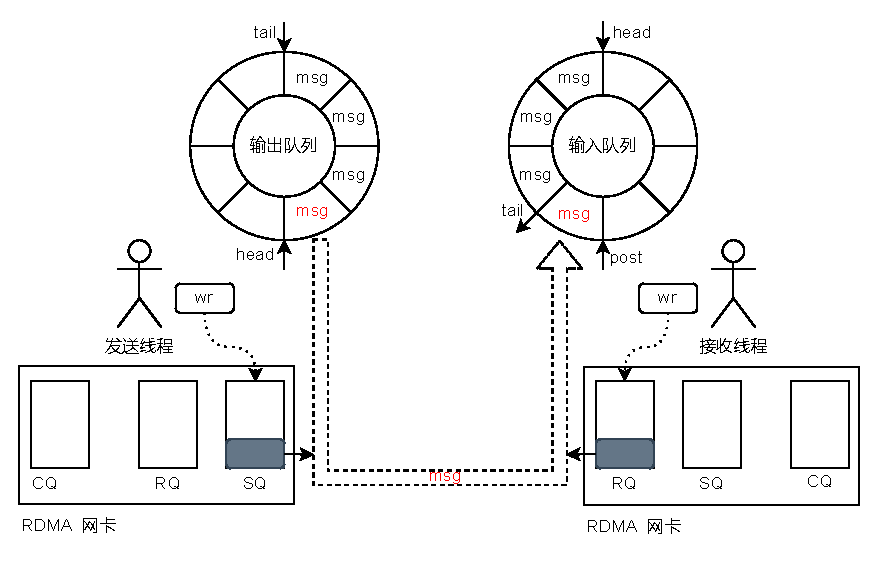
\includegraphics[width=\textwidth]{Img/RDMA通信栈可靠链接.drawio.pdf}
        \bicaption{\enspace RDMA 通信栈可靠连接 Send 示例}{\enspace RDMA communication stack reliable connection Send example}
        \label{fig:mjiajia-send-recv}
    \end{figure}



    \subsection{RDMA 通信管理器设计}

    M-JIAJIA 的 RDMA 通信管理器(jia\_context\_t)旨在管理 RDMA 通信所涉及的资源和配置参数。具体可分为以下几部分:

    \begin{enumerate}[label=\arabic*., leftmargin=1em, align=left]
        \item \textbf{RDMA 设备相关信息}
              \begin{itemize}
                  \item \textbf{设备上下文}:设备上下文是应用程序与 RDMA 硬件之间的接口,用于管理所有其他 RDMA 资源。
                  \item \textbf{设备端口号}:设备端口号用于标识 RDMA 设备进行通信的物理端口。
              \end{itemize}

        \item \textbf{RDMA 资源管理信息}
              \begin{itemize}
                  \item \textbf{保护域}:保护域(Protect Domain, PD)是一种资源隔离手段,在RC 模式下用于限制 QPs 可以访问内存区域(Memory Region,MR)的范围。
                  \item \textbf{内存区域}:内存区域是应用程序注册后可被 RDMA 设备直接访问的内存。M-JIAJIA 采用 Send 原语进行通信,因此需分别为发送和接收准备独立的内存区域。在多通信场景下,考虑到输入的不确定性,M-JIAJIA 采用单输出、多输入的内存区域设计方案。
              \end{itemize}

        \item \textbf{RDMA 事件通知信息}
              \begin{itemize}
                  \item \textbf{完成事件通道}:完成事件通道提供 CQ 事件通知机制,用于通知工作请求是否完成。M-JIAJIA 提供独立的发送和接收完成事件通道。
              \end{itemize}

        \item \textbf{RDMA 连接管理信息}
              \begin{itemize}
                  \item \textbf{RDMA 连接管理结构}:该结构用于管理与每个连接相关的信息。包括连接状态、发送序号和接收序号、RDMA 连接管理标识符(rdma\_cm\_id)、输入队列和输入内存区域。
                  \item \textbf{RDMA 连接管理结构数组}:连接管理结构数组记录了与每个远端节点的连接信息。
                  \item \textbf{RDMA 建立连接线程标识}:M-JIAJIA 采用客户端-服务器模式建立连接。在建连阶段,节点分别创建客户端和服务器线程以完成连接。其建连方案具有独特性:每个节点至多创建一个服务器线程用于监听连接请求,同时可创建多个客户端线程主动发起连接。线程标识用于存储和管理线程的信息,便于线程创建、同步和管理。
              \end{itemize}
    \end{enumerate}

    \subsection{RDMA 通信栈组成模块}

    为构建基于 RDMA 可靠连接(RC)的通信系统,RDMA 通信栈的初始化流程分为以下四个主要阶段(如图~\ref{fig:mjiajia-rdma-modules}右侧所示):
    \begin{enumerate}[label=\arabic*.]
        \item 初始化上下文。包括获取设备列表、选择硬件设备、打开设备获取上下文、配置物理端口以及输入/输出消息队列初始化等步骤。
        \item 建立连接。通过创建线程向其他主机发起建连请求、并响应其他主机的连接请求,完成任意两节点之间的建连。
        \item 初始化通信资源。主要用于注册输入/输出内存区域(MR)。
        \item 多线程通信。创建线程分别负责下发发送/接收工作请求(WR),同时创建专门处理消息的线程,以优化通信效率。
    \end{enumerate}

    \begin{figure}[!htbp]
        \centering
        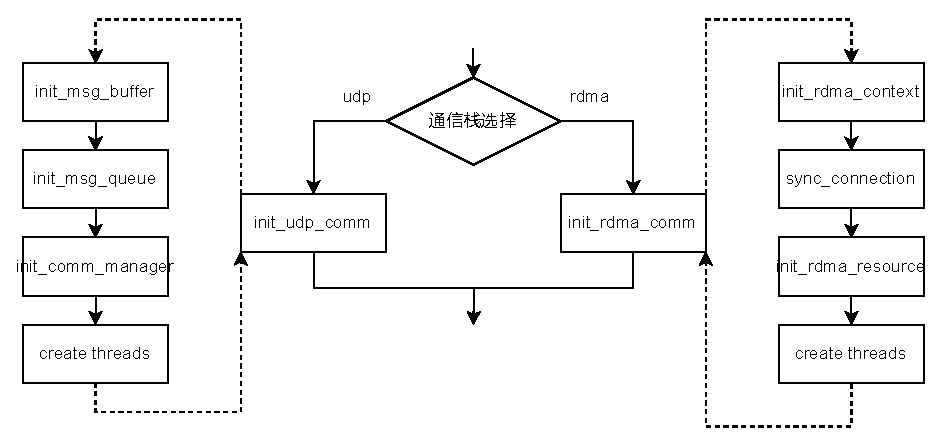
\includegraphics[width=\textwidth]{Img/MJIAJIA通信栈.drawio.pdf}
        \bicaption{\enspace M-JIAJIA 通信栈}{\enspace M-JIAJIA communication stack}
        \label{fig:mjiajia-rdma-modules}
    \end{figure}

    \section{可靠通信连接建立机制}\label{sec:可靠通信连接建立机制}
    M-JIAJIA 采用基于 RDMA CM 的建连方式。该方式具有三个显著优势:
    \begin{enumerate}[label=\arabic*.]
        \item 编程简单,RDMA CM 封装了底层复杂的连接建立过程,使开发者无需直接操作Verbs API即可完成通信流程。
        \item 开销低,RDMA CM 支持异步操作模式,通过事件通道(Event Channel)实现非阻塞通信,避免轮询带来的开销。
        \item 可移植性强,RDMA CM 兼容InfiniBand、RoCEV2和iWARP多种 RDMA 实现,无需针对不同硬件进行代码修改。
    \end{enumerate}

    如图~\ref{fig:mjiajia-cm-connection}所示,建连过程需要客户端和服务器紧密配合,共同完成一系列复杂的步骤,最终生成用于通信的 rdma\_cm\_id 。

    \begin{figure}[H]
        \centering
        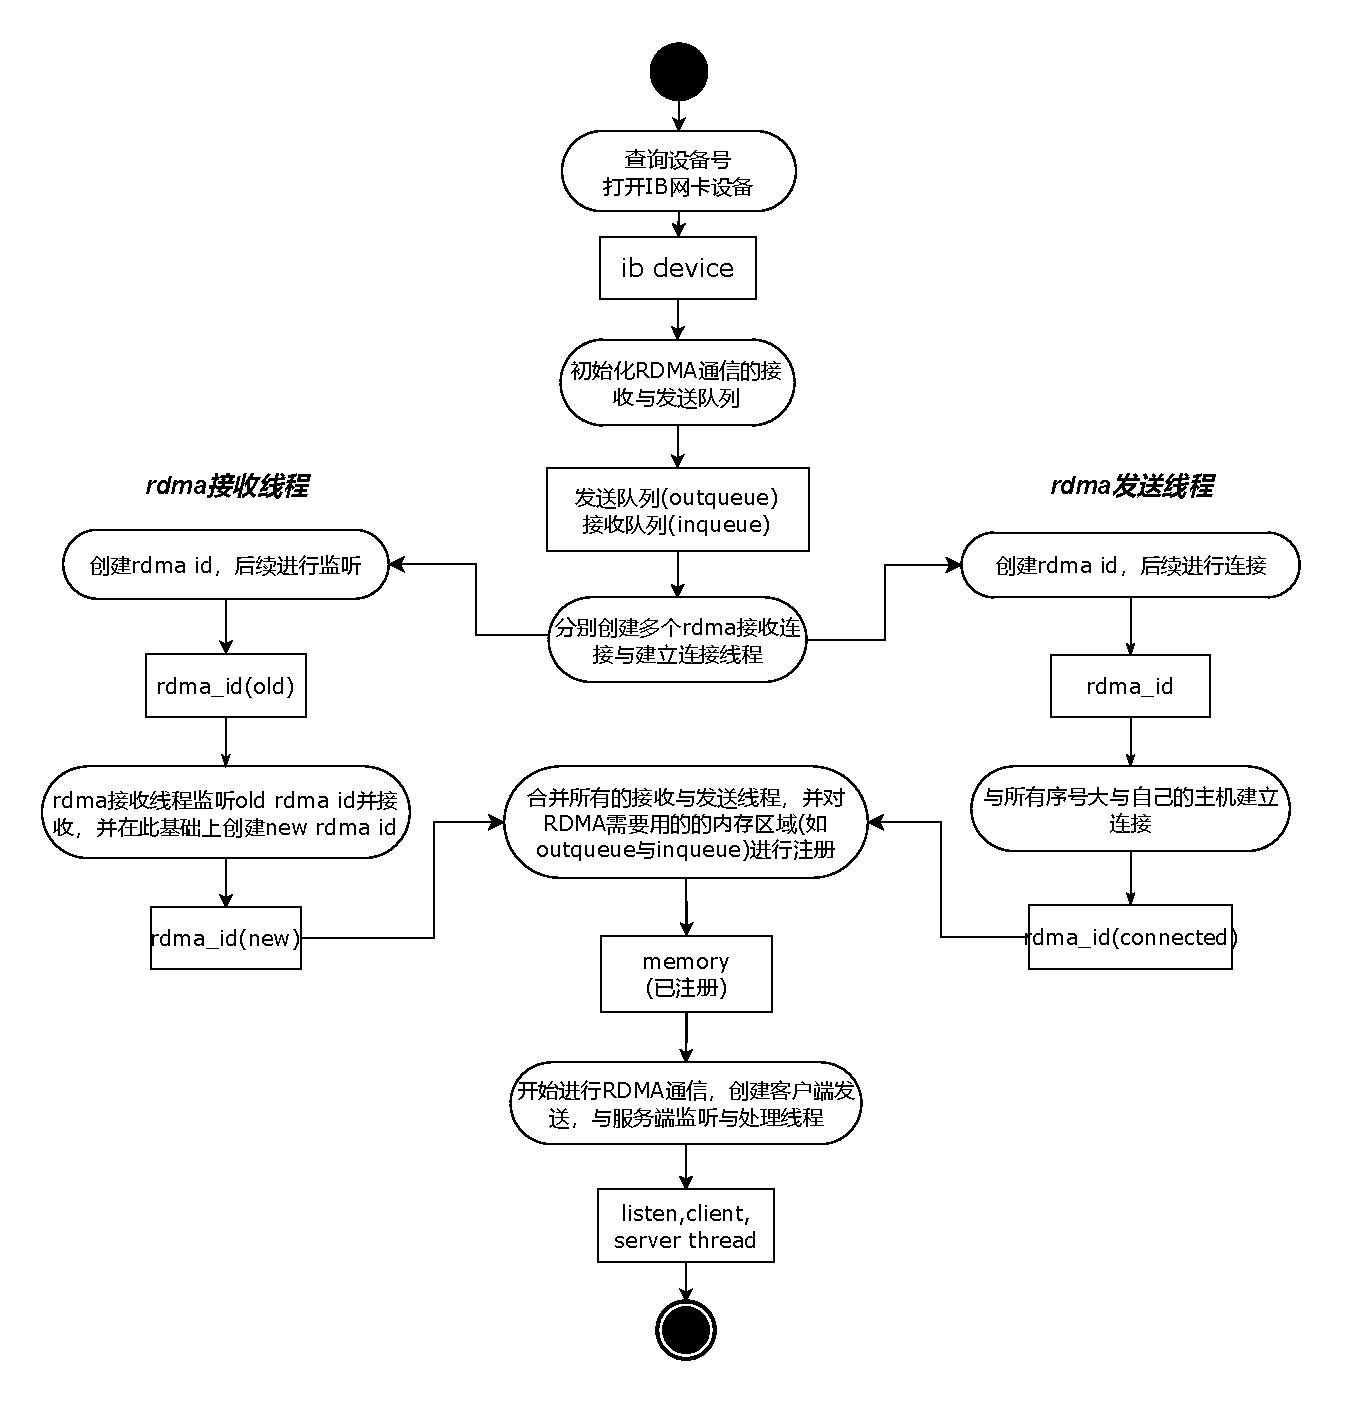
\includegraphics[width=\textwidth]{Img/rdma_init.drawio.pdf}
        \bicaption{M-JIAJIA RDMA CM 建连流程图}{M-JIAJIA RDMA CM Connection Establishment Flowchart}
        \label{fig:mjiajia-cm-connection}
    \end{figure}

    \subsection{RDMA 集群建连算法}

    M-JIAJIA 运行时要求任意两节点具备通信能力,因此必须在任意两节点之间至少建立一个连接。
    M-JIAJIA 采用客户端服务器模式,通过创建多个客户线程与服务线程去建立连接,并采用了算法~\ref{alg:connection-algo}所示的建连算法,
    不必为每个连接设立单独的服务器处理。

    在rdma同步的过程中,主机号偏小的主机会创建多个client线程与主机号偏大的主机server线程尝试建立连接;
    同时除jia\_pid为0外所有的主机都会创建一个server线程来监听建立的rdma连接,最终每两台主机之间建立一个rdma连接;
    如图~\ref{fig:RDMA-connection-build}所示,创建线程并建立连接。

    \begin{figure}[H]
        \centering
        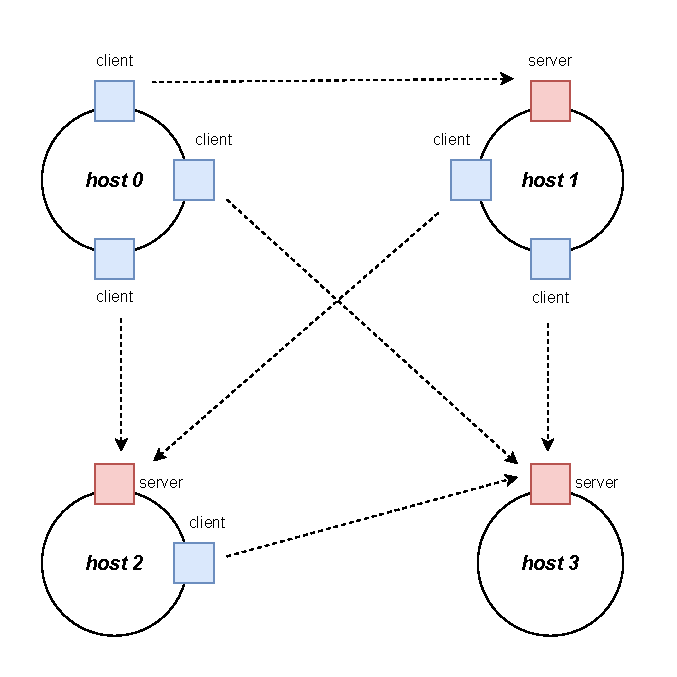
\includegraphics[width=0.65\textwidth]{Img/rdma_sync.drawio.pdf}
        \bicaption{\enspace RDMA集群建连示例}{\enspace RDMA Cluster Connection Establishment Example}
        \label{fig:RDMA-connection-build}
    \end{figure}

    \begin{algorithm}
        \caption{RDMA Cluster Connection Establishment Algorithm}\label{alg:connection-algo}
        \begin{algorithmic}[1]
            \Procedure{sync\_connection}{$hosts$, $pid$}
            \If{$pid$ $\neq$ 0}
            \State \Call{pthread\_create}{\&ctx.server\_thread, NULL, server\_thread, \&ctx}
            \EndIf
            \State $num\_clients$ $\gets$ $hosts$ - $pid$ - 1
            \If{$num\_clients$ $>$ 0}
            \State $ctx.client\_threads$ $\gets$ \Call{malloc}{$num\_clients$ * sizeof(pthread\_t)}
            \For{$i \gets 0$ to $num\_clients$}
            \State $target\_hosts$ $\gets$ \Call{malloc}{sizeof(int)}
            \State $*target\_hosts$ $\gets$ $pid + i + 1$
            \State \Call{pthread\_create}{\&ctx.client\_threads[i], NULL, client\_thread, target\_hosts}
            \EndFor
            \EndIf
            \If{$pid$ $\neq$ 0}
            \State \Call{pthread\_join}{ctx.server\_thread, NULL}
            \EndIf

            \If{$num\_clients$ > 0}
            \For{$i \gets 0$ to $num\_clients$}
            \State \Call{pthread\_join}{ctx.client\_threads[i], NULL}
            \EndFor
            \EndIf
            \EndProcedure
        \end{algorithmic}
    \end{algorithm}

    \section{RDMA 多线程通信架构设计}\label{sec:RDMA 多线程通信架构设计}

    \begin{figure}[H]
        \centering
        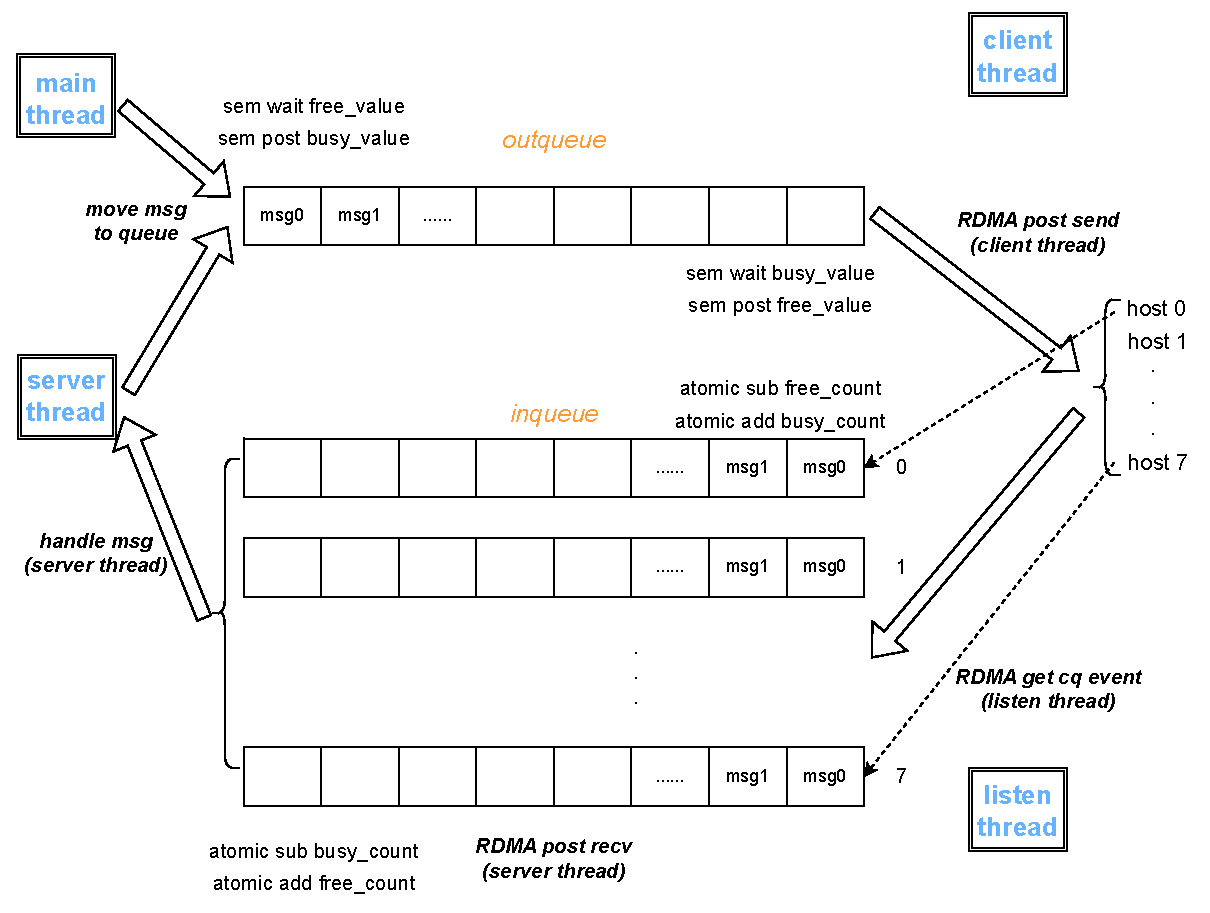
\includegraphics[width=1.1\textwidth]{Img/RDMA_design.drawio.pdf}
        \bicaption{\enspace RDMA通信设计}{RDMA communication design}
    \end{figure}


    \subsection{RDMA 多线程任务划分}

    \subsubsection{RDMA通信接收端线程任务划分}
    RDMA通信接收端由listen与server两个线程组成,他们的任务划分如下:

    \begin{itemize}[leftmargin=*, nosep]
        \item \textbf{listen thread}:
              轮询或事件通知机制检测Recv操作的完成状态,检测到Recv操作完成时通知server线程进行处理;
        \item \textbf{server thread}:
              初始化时,预先为每个QP下发多个Recv Buffer用于预备接收;
              在得到listen thread通知后,从inqueue中取出消息进行处理,同时继续下发新的Recv请求,
              确保始终有足够的Recv Buffer接收后续的消息;
    \end{itemize}

    \begin{figure}[H]
        \centering
        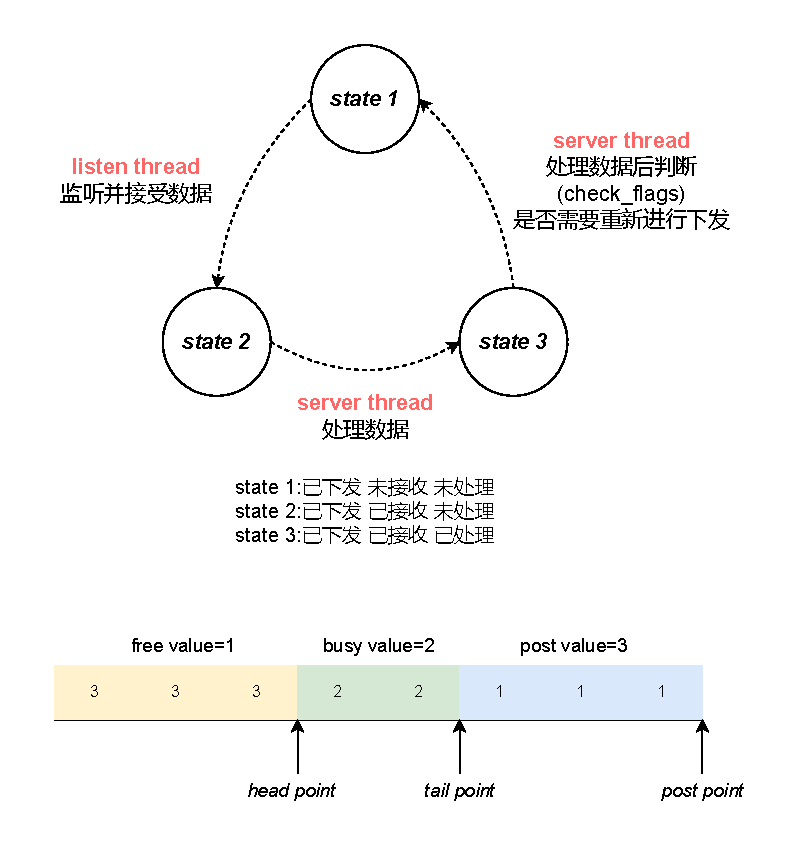
\includegraphics[width=1.0\textwidth]{Img/recv_state.drawio.pdf}
        \bicaption{RDMA接收端inqueue中msg的状态转换}{RDMA recv state change}
    \end{figure}

    listen thread的伪代码如下:
    \begin{algorithm}
        \caption{listen thread algorithm}
        \begin{algorithmic}[1] % [1] 使得每行都有行        
            \Procedure{ListenThread}{}
            \State \Call{post\_recv}{$ $}
            \State \textbf{return} NULL
            \EndProcedure

            \Function{post\_recv}{}
            \While{$true$}
            \State $\{ cq\_ptr, context\} \gets$ \Call{ibv\_get\_cq\_event}{$recv\_comp\_channel$}
            \State $inqueue \gets (rdma\_connect\_t)context.inqueue$
            \State \Call{ibv\_req\_notify\_cq}{$cq\_ptr$}
            \State $wc \gets$ \Call{ibv\_poll\_cq}{$cq\_ptr$}

            \State
            \If{$wc.status \neq \text{IBV\_WC\_SUCCESS}$}
            \State \Call{log\_err}{$post\_recv \quad error$}
            \Else
            \State \Call{atomic\_fetch\_sub}{$inqueue$->$post\_value$}
            \State \Call{atomic\_fetch\_add}{$inqueue$->$busy\_value$}

            \State
            \State $connect\_array[inqueue$->$queue[inqueue$->$tail]$->$topid].rcv\_seq $++
            \State $inqueue$->$tail \gets (inqueue$->$tail$+1$) \% QueueSize$
            \EndIf
            \EndWhile

            \State
            \State \Call{ibv\_ack\_cq\_events}{$cq\_ptr$}
            \State \textbf{return}
            \EndFunction
        \end{algorithmic}
    \end{algorithm}

    \newpage
    server thread的伪代码如下:
    \begin{algorithm}
        \caption{server thread algorithm}
        \begin{algorithmic}[1] % [1] 使得每行都有行号
            \Procedure{ServerThread}{}
            \State \Call{init\_post\_recv\_wr}{$ $}

            \While{$true$}
            \For{$i \gets 0$ to $hostc$}
            \State $tmp\_connect \gets connect\_array[i]$
            \State $in\_queue \gets tmp\_connect$->$inqueue$
            \If{\Call{atomic\_load}{$tmp\_connect.inqueue$->$busy\_value$}}
            \State \Call{msg\_handle}{$inqueue$->$queue[head]$}
            \State \Call{atomic\_fetch\_sub}{$inqueue$->$busy\_value$}
            \State \Call{atomic\_fetch\_add}{$inqueue$->$free\_value$}
            \If{$i == jia\_pid$}
            \State $tmp\_connect.rcv\_seq$ ++
            \EndIf
            \State $inqueue$->$head \gets (inqueue$->$head$+1$) \% QueueSize$
            \EndIf
            \EndFor

            \If{$i \neq jia\_pid$}
            \State \Call{check\_flags}{$i$}
            \EndIf
            \EndWhile
            \State \textbf{return}
            \EndProcedure
        \end{algorithmic}
    \end{algorithm}

    \newpage
    \subsubsection{RDMA通信发送端线程任务划分}
    RDMA通信接收端由main/server两个入队线程,和一个client发送线程组成,他们的任务划分如下:

    \begin{itemize}[leftmargin=*, nosep]
        \item \textbf{main/server thread}:
              用于下发rdma需要发送的msg,并将msg放入outqueue队列中,
              队列中的每个消息包含目标主机的IP地址和消息内容;
        \item \textbf{client thread}:
              将对应的msg从outqueue队列中取出,
              并调用\texttt{ibv\_post\_send} API发送msg给对应主机;
              发送后发送端通过轮询或事件通知机制(如Completion Queue)检测Send操作的完成状态,操作失败则记录错误日志。
    \end{itemize}

    \begin{figure}[H]
        \centering
        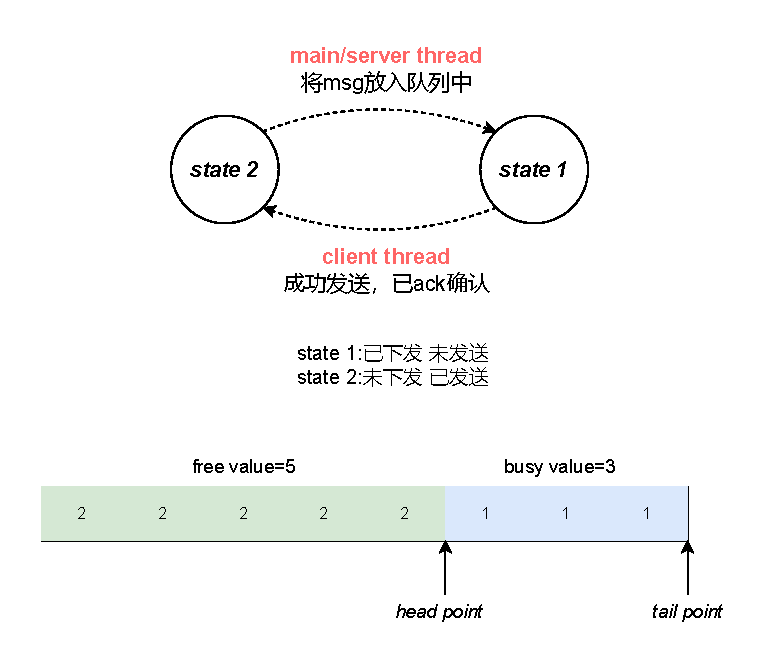
\includegraphics[width=1.0\textwidth]{Img/send_state.drawio.pdf}
        \bicaption{RDMA发送端outqueue中msg的状态转换}{RDMA send state change}
    \end{figure}

    client thread的伪代码如下:
    \begin{algorithm}
        \caption{client thread algorithm}
        \begin{algorithmic}[1] % [1] 使得每行都有行号
            \Procedure{ClientThread}{}
            \While{$true$}
            \State \Call{sem\_wait}{$outqueue.busy\_count$}
            \State $msg\_ptr \gets$ \Call{dequeue}{$outqueue$}
            \State $msg\_ptr$->$seqno \gets connect\_array[msg\_ptr$->$to\_pid]$

            \State
            \If{$msg\_ptr$->$topid$ = $jia\_pid$}
            \State \Call{memcpy}{$inqueue[tail],msg\_ptr$}
            \State \Call{atomic\_fetch\_sub}{$inqueue$->$free\_value$}
            \State \Call{atomic\_fetch\_add}{$inqueue$->$busy\_value$}
            \State $inqueue$->$tail \gets (inqueue$->$tail$+1$) \%QueueSize$
            \Else
            \While{\Call{post\_send}{$connect\_array[msg\_ptr$->$to\_pid]$}}
            \EndWhile
            \EndIf

            \State
            \State $connect\_array[msg\_ptr$->$topid].snd\_seq$++
            \State $inqueue$->$head \gets (inqueue$->$head$+1$) \% QueueSize$
            \State \Call{sem\_post}{$outqueue.free\_count$}
            \EndWhile
            \State \textbf{return}
            \EndProcedure
        \end{algorithmic}
    \end{algorithm}

    \section{本章小结}
    本章 \ref{sec:RDMA设计概览} 节介绍了 M-JIAJIA RDMA通信模式与通信原语选择,并给出了 M-JIAJIA 中RDMA管理器的基本设计与组成模块。

    本章 \ref{sec:可靠通信连接建立机制} 节介绍了 M-JIAJIA RDMA基本的建连过程和对应的算法。

    本章 \ref{sec:RDMA 多线程通信架构设计} 节介绍了 M-JIAJIA 多线程的任务划分算法,以及接收端发送端每个msg slot的状态转换。
}